
\section{Pointer-Chasing Data Structure}
\label{section:pointer_chasing}
In a pointer-chasing data structure, an operation to the data structure has to 
traverse over the data structure, following a sequence of pointers, before it completes.
The examples we consider in the paper are linked-list and skip-list,
where add($x$), delete($x$) and contains($x$) operations have to go through
a sequence of ``next node" pointers until reaching the position of node $x$.

In a pointer-chasing data structure,
the performance bottleneck is the procedure of the pointer chasing of operations.
We focus on data structures much larger than the size of cache of CPUs
such that a large portion of a data structure has to resides in memory at any time.
Thus, the performance bottleneck of such a data structure is
the memory accesses incurred during pointer chasing.


\subsection{PIM-managed linked-list}
\label{section:linked_list}
The naive PIM-managed linked-list is simple:
the linked-list is stored in a vault, maintained by the local PIM core.
Whenever a CPU wants to make an operation to the linked-list,
it sends the PIM core a message containing a request of the operation
and the PIM core will later retrieve the message and execute the operation.
The concurrent linked-list can actually be implemented
as a sequential linked-list, since it is accessible directly only by the PIM core.

Doing pointer chasing on sequential data structures by PIM cores is not a new idea
(e.g., \cite{hsieh2016accelerating, Ahn2015:2}).
It is obvious that for a sequential data structure like a sequential linked-list,
replacing the CPU with a PIM core to access the data structure will largely improve
its performance due to the PIM core's much faster memory access.
However, we are not aware of any prior comparison between the performance of
PIM-managed data structures and concurrent data structures
in which CPUs can make operations in parallel.
In fact, our analytical and experimental results will show that
the performance of the naive PIM-managed linked-list is much worse than
that of the concurrent linked-list with fine-grained locks\cite{Heller05}.

To improve the performance of the PIM-managed linked-list,
we can apply the following \emph{combining optimization} to it:
The PIM core retrieves all operation requests from its buffer and
execute all of them during only one traversal over the linked-list.

It is not hard to see that the role of the PIM core in our PIM-managed linked-list
is very similar to that of the combiner in a concurrent linked-list implemented
using flat combining \cite{Hendler10}, where, roughly speaking,
threads (CPUs) compete for a ``combiner lock" to become the combiner, and
the combiner will take over all operation requests from other CPUs and execute them.
Hence, we think the performance of the flat-combining linked-list is a good indicator to
the performance of our PIM-managed linked-list.

Based on our performance model, we can calculate the approximate expected
throughputs of the linked-list algorithms mentioned above, 
when there are $p$ CPUs making operation requests concurrently.
We assume a linked-list consists of nodes whose keys are integers in the range of $[1, N]$.
Initially a linked-list has $n$ nodes with keys generated independently
and uniformly at random from $[1, N]$.
The keys of the operation requests of the CPUs are generated the same way.
To simplify the calculations, we assume CPUs only make contains() requests
(or the number of $add()$ requests is almost the same as the number of $delete()$
so that the size of each linked-list nearly doesn't change).
We also assume that a CPU makes a new operation request immediately after
its previous one completes.
The approximate expected throughputs (per second) of the concurrent linked-lists
are as follows, given $n >> p$ and $N >> p$.

\begin{itemize}
\item Concurrent linked-list with fine-grained locks:
	${2p \over (n+1)\latcpu}$

\item Flat-combining linked-list without combining optimization:
	${2 \over (n+1)\latcpu}$

\item PIM-managed linked-list without combining optimization:
	${2 \over (n+1)\latpim}$

\item Flat-combining linked-list with combining optimization:
    ${p \over (n-\Sp)\latcpu}$

\item PIM-managed linked-list with combining optimization:
    ${p \over (n-\Sp)\latpim}$
\end{itemize}

where $\Sp = \sum\limits_{i=1}^{n} ({i \over n+1})^{p}$.\footnote {
We define the rank of an operation request to a linked-list as the number of pointers
we have to traverse until we find the right position for it in the linked-list.
$\Sp$ is actually the expected rank of the operation request with the biggest key
among $p$ random requests a PIM core or a combiner has to combine,
which is essentially the expected number of pointers a PIM core or a combiner
has to go through during the pointer chasing procedure.}

Since $0 < \Sp \le {n \over 2}$ and $\latcpu = 3\latpim$,
it is not hard to see that the PIM-managed linked-list with
combining optimization outperforms all other algorithms
(in fact its throughput is at least 1.5 times the throughput of
the second best algorithm, the one with fine-grained locks).
Without combining, however, the PIM-managed linked-list cannot
beat the linked-list with fine-grained locks when $p > 6$.

We have implemented the linked-list with fine-grained locks
and the flat-combining link-list with and without combining optimization.
We have run them on a node of 28 hardware threads in a machine
and their throughputs are presented in Figure \ref{figure:linkedlist_data}.
The results meet our expectation based on the analytical results above.
The throughput of the flat-combining algorithm without combining optimization
is much worse than the algorithm with fine-grained locks.
According to our analytical results, we triple the throughput of the
flat-combining algorithm without combining optimization to get the estimated
throughput of the PIM-managed algorithm. As we can see,
it is still far away from the throughput of the one with fined-grained locks.
However, with combining optimization, the performance of the flat-combining
algorithm improves significantly and the estimated throughput of our PIM-managed
linked-list with combining optimization finally beats all others'.

\begin{figure}[ht!]
%$\hrulefill$
%\\
%\\
\centering
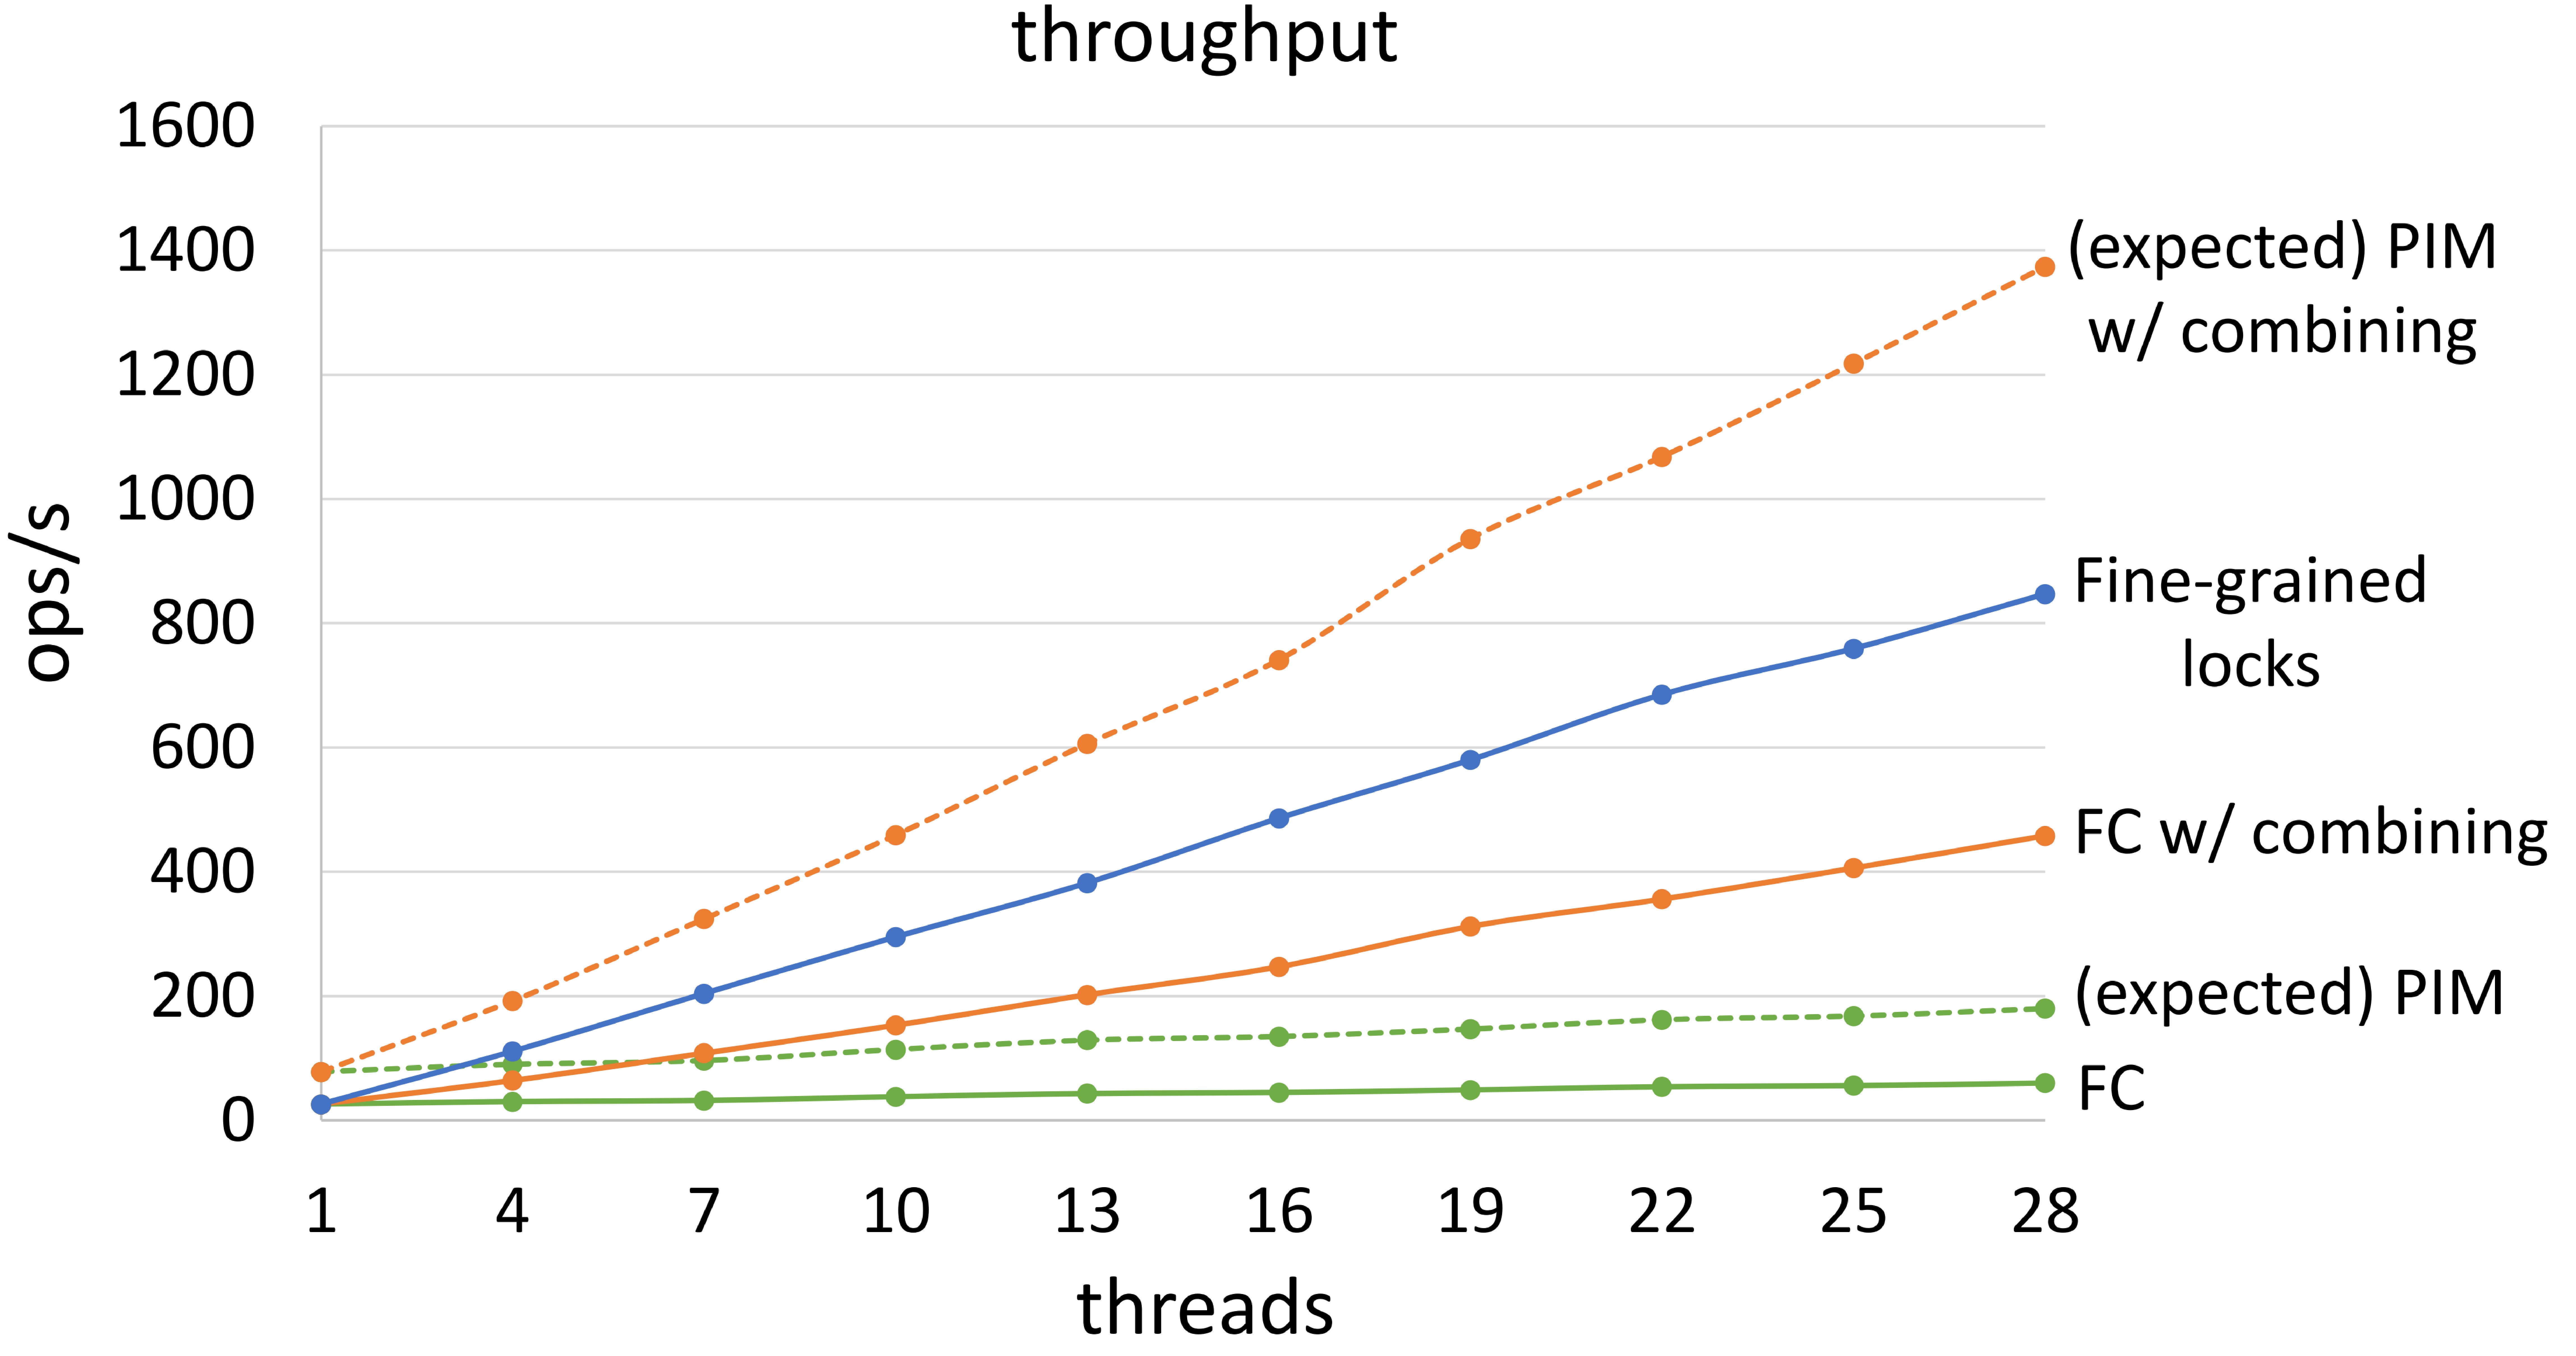
\includegraphics[width=.8\linewidth]{linkedlist_data.eps}
%$\hrulefill$
\caption{Experimental results of linked-lists}
\label{figure:linkedlist_data}
\end{figure}

\subsection{PIM-managed skip-list}
\label{section:skip_list}

\subsubsection{Base algorithm}
Like the naive PIM-managed linked-list,
the naive PIM-managed skip-list keeps the skip-list in a single vault and
CPUs send operation requests to the local PIM core which executes those operations.
As we will see, this algorithm is less efficient than some existing algorithms either.

Unfortunately, the combining optimization cannot be applied to skip-lists effectively.
The reason is that for any two nodes not close enough to each other in the skip-list,
the paths we traverse through to reach them don't largely overlap.

On the other hand, PIM memory usually consist of many vaults and PIM cores.
For instance, the first generation of Hybrid Memory Cube \cite{website:HMC} has 32 vaults.
Hence, a PIM-managed skip-list may achieve much better performance if
we can exploit the parallelism of multiple vaults and PIM cores.
Here we present our PIM-managed skip-list with \emph{partitioning optimization}:
A skip-list is divided into partitions of disjoint ranges of keys,
stored in different vaults, so that a CPU sends its operation request to
the PIM core of the vault to which the request belongs.

Figure \ref{figure:skiplist_structure} illustrates the structure of a PIM-managed skip-list.
Each partition of a skip-list starts with a \emph{sentinel node}
which is a node of the max height. For simplicity, assume the max height $H_{max}$ 
is predefined and each node in a skip-list has height between 1 and $H_{max}$.
The key range a partition covers is the between the key of its sentinel node and
the key of the sentinel node of the next partition.

CPUs also store a copy of each sentinel node in the normal DRAM of the PIM memory 
and the copy has an extra variable indicating the vault containing the sentinel node.
Since the number of nodes of the max height is very small with high probability, 
the copies of those sentinel nodes can almost for certain stay in cache
if CPUs access them frequently.

When a CPU wants to make an operation of some key to the skip-list,
it first compares the key with those of the sentinels, finds out the vault
the key belongs to, and then sends its operation request to
the PIM core of the vault.
Once the PIM core retrieves the request, it executes the operation in the local vault 
and finally sends the result back to the CPU.


\begin{figure}[ht!]
%$\hrulefill$
%\\
%\\
\centering
\includegraphics[width=.8\linewidth]{skiplist_structure.eps}
%$\hrulefill$
\caption{A PIM-managed FIFO queue with three partitions}
\label{figure:skiplist_structure}
\end{figure}

Now let us discuss how to implement our PIM-managed skip-list
when the key of each operation is an integer generated uniformly at random
from range $[0, n]$ and the PIM memory has $k$ vaults available.
In this case, we can initialize $k$ partitions starting with fake sentinel nodes
$0, 1/k, 2/k,..., (n-1)/k$, respectively.
We allocate one partition in a different vault and hence $k$ vaults cover
$k$ disjoint key ranges of size same.
The sentinel nodes will never be deleted.
If a new node to be added has the same key as a sentinel node,
we add it immediately after the sentinel node.

We compare the performance of our PIM-managed skip-list with partitions 
with the performance of a flat-combining skip-list \cite{Hendler10} with modifications
and a lock-free skip-list \cite{Herlihy08}, 
in a machine with $p$ CPUs and $k$ PIM vaults.
To simplify the comparison, we assume that all skip-lists have the same
initial structure (expect that skip-lists with partitions have extra sentinel nodes)
and all the operations are contains() operations
(or the number of $add()$ requests is almost the same as the number of $delete()$ 
so that the size of each skip-list nearly doesn't change).
Their approximate expected throughputs are as follows:

\begin{itemize}
\item Look-free skip-list:
	${p \over \beta\latcpu}$

\item Flat-combining skip-list without partitioning:
	${1 \over \beta\latcpu}$

\item PIM-managed skip-list without partitioning:
	${1 \over (\beta\latpim + \latmes)}$

\item Flat-combining skip-list with $k$ partitions:
    ${k \over \beta\latcpu}$

\item PIM-managed linked-list with $k$ partitions:
    ${k \over (\beta\latpim + \latmes)}$
\end{itemize}

where $\beta$ is the average number of nodes an operation has to go through
in order to find the location of its key in a skip-list
($\beta = \Theta(\log N)$, where $N$ is the size of the skip-list).
The flat-combining skip-list with $k$ partitions is one that has $k$ combiner locks,
each for a partition, so that CPUs compete for locks of partitions their operation
keys belong to.
Note that in the analysis above, we ignored some overheads in the flat-combining
algorithms, such as maintaining combiner locks and publication lists
(we will discuss publication lists in more detail in Section \ref{section:contended}).
We also overestimated the performance of the lock-free skip-list by not counting the
CAS operations used in add() and delete() requests, as well as the cost of retries
caused by conflicts of updates.
Even so, our PIM-managed linked-list with partitioning optimization is
still expected to outperformance other algorithms when $k > p/3$.

Our experiments have revealed similar results, 
as presented in Figure \ref{figure:skiplist_data}.
We have implemented and run the flat-combining skip-list with different numbers of
partitions and compared them with the lock-free skip-list.
As the number of partitions increases, the performance of the flat-combining skip-list
gets better and better, implying the effectiveness of partitioning optimization.
Again we believe the performance of the flat-combining skip-list is a good indicator
to the performance of our PIM-managed skip-list.
Therefore, according to the analytical results we have shown, we can triple the throughput
of a flat-combining skip-list to get the expected performance of a PIM-managed skip-list.
As the figure illustrates, when the PIM-managed skip-list has $8$ or $16$ partitions,
it is expected to outperform the lock-free skip-list with up to 28 hardware threads.

\begin{figure}[ht!]
%$\hrulefill$
%\\
%\\
\centering

\includegraphics[width=.8\linewidth]{skiplist_data.eps}
%$\hrulefill$
\caption{Experimental results of skip-lists}
\label{figure:skiplist_data}
\end{figure}

\subsubsection{Rebalancing skip-list}
We have shown that our PIM-managed skip-list performs well with uniform distribution of requests. 
With non-uniform distribution of requests, we may need to periodically rebalance the skip-list 
in order to maintain good performance. 
Here we discuss how to migrate consecutive nodes from one vault to another without blocking requests.  

To move consecutive nodes from its local vault to another vault $v$, a PIM core $p$ 
can send messages of requests of adding those nodes to the local PIM core $q$ of $v$ as follows. 
First, $p$ sends a message notifying $q$ of the start of the node migration. 
Then $p$ sends messages of adding those nodes to $q$ one by one in an ascending order 
according to the keys of the nodes. 
After all those nodes have been migrated, $p$ sends notification messages to CPUs so that 
CPUs can update their copies of sentinel nodes accordingly.
Once $p$ receives acknowledgement messages from all CPUs, it notifies $q$ of the end of migration.
To keep the node migration protocol simple, we don't allow $q$ to move those nodes 
to another vault again until $v$ finishes its node migration. 

During this node migration, $p$ can periodically check its message buffer for requests from CPUs.
Assume that a request with key $k_1$ is sent to $p$ when $p$ is migrating nodes 
in a key range that $k_1$ is in.  
If $p$ is about to send a message to migrate a node with $k_2$ at the moment, where $k_1 \ge k_2$, 
$p$ serves the request itself. 
Otherwise $p$ forwards the request to $q$. 
In either case, $p$ can then continue its node migration without blocking concurrent requests. 
It is not hard to see the correctness of the node migration procedure 
with the presence of requests: a request will eventually reach the vault that 
currently contains nodes in the key range that the request is in.
If a request later arrives to $p$ which no longer holds the partition the request belongs to, 
$p$ can simply reply with a rejection to the sender CPU and 
the sender CPU will resend its request to the correct PIM core, 
because the CPU has already updated its sentinels and knows which PIM core it should contact. 

Using this node migration protocol, our FIFO queue can support two rebalancing schemes:
1) If a partition has too many nodes, the local PIM core can divide it into two smaller  
partitions (the first nodes of two smaller partitions are modified to have the max height 
in order to serve as sentinels) and migrate one of them to another PIM vault; 
2) If two consecutive partitions are both small, we can merge then by moving one to the vault 
containing the other. 
If rebalancing happens infrequently, its overhead is affordable. 
